\documentclass[9pt,twocolumn]{opticajnl}
\journal{opticajournal}
\setboolean{shortarticle}{true}
\IfFileExists{siunitx.sty}{%
  \usepackage{siunitx}
  \sisetup{range-phrase = --, range-units = single}
  \sisetup{per-mode = symbol}
}{%
  \newcommand{\sisetup}[1]{}
  \newcommand{\SI}[2]{\ensuremath{##1\,##2}}
  \newcommand{\SIrange}[3]{\ensuremath{##1\text{--}##2\,##3}}
  \newcommand{\DeclareSIUnit}[2]{}
}
\providecommand{\nano}{\ensuremath{\mathrm{n}}}
\providecommand{\micro}{\ensuremath{\mu}}
\providecommand{\milli}{\ensuremath{\mathrm{m}}}
\providecommand{\second}{\ensuremath{\mathrm{s}}}
\providecommand{\meter}{\ensuremath{\mathrm{m}}}
\providecommand{\per}{\ensuremath{\,/\,}}
\providecommand{\pixel}{\ensuremath{\mathrm{px}}}
\providecommand{\USD}{\ensuremath{\mathrm{USD}}}
\DeclareSIUnit{\pixel}{px}
\DeclareSIUnit{\USD}{USD}



% \title{Self-synchronized event-driven transmission hyperspectral imaging with multi-window scanning compensation}
\title{Self-Calibrated Neuromorphic Hyperspectral Sensing}
\author[]{Rongzhou Chen}
\author[]{Chutian Wang}
\author[]{Yuqing Cao}
\author[*]{Edmund Y. Lam}
\affil[]{Department of Electrical and Electronic Engineering, The University of Hong Kong, Pokfulam, Hong Kong, China}
\affil[*]{elam@eee.hku.hk}
\dates{\today}
\ociscodes{Multispectral and hyperspectral imaging; Instrumentation, measurement, and metrology; Image reconstruction techniques; Computational imaging}
\doi{\url{}}

\begin{abstract}
We demonstrate a transmission hyperspectral system that drives a diffracted illumination across a specimen and records the induced intensity dynamics with an event camera. Instead of relying on calibrated motor encoders or trigger wiring, the method self-synchronizes the scan by analysing the event activity via auto-correlation and correlation with its own reversal auto-convolution, yielding forward and backward segmentation directly from the data stream. A multi-window compensation model with soft spatial memberships then compensates acceleration-induced temporal shear by minimizing within-bin event variance, outperforming single velocity corrections under low-cost motor actuation. The reconstructed spectra match a reference hyperspectral camera even in low-light conditions where the frame-based sensor degrades, underlining the advantage of the event-based imaging. 
\end{abstract}

\usepackage{ifthen}
\usepackage{placeins}
\usepackage{xcolor}
\usepackage{tikz}
\usetikzlibrary{arrows.meta,positioning,shadings}
% Colors used in event cloud legends
\definecolor{evtPos}{HTML}{FFBB78} % +1 polarity (orange)
\definecolor{evtNeg}{HTML}{AEC7E8} % -1 polarity (blue)

% Yellow placeholder figure macro for drafts
\newcommand{\phfig}[2][0.95\linewidth]{%
  \begingroup\setlength{\fboxsep}{0pt}\colorbox{yellow!20}{%
    \parbox{#1}{\vspace{16mm}\centering\textbf{PLACEHOLDER}\\\small #2\vspace{14mm}}}%
  \endgroup}

\providecommand{\nocitefullrefs}[1]{}


\begin{document}

\maketitle

\newcommand{\olsection}[1]{\par\noindent\textbf{#1.} }

\olsection{Introduction}
Scanning hyperspectral imagers deliver high spectral resolution at the expense of mechanical complexity and strict synchronization between motion and detection elements~\cite{hagen2013review}. Conventional systems integrate encoder signals, tachometers, or trigger lines to maintain spatial--spectral registration, which complicates low-cost deployments and long-term stability~\cite{yeh2011selfcal,alhourani2023linescan}. Event cameras provide an alternative sensing modality: they asynchronously report logarithmic intensity changes with microsecond latency and high dynamic range, recording only the temporal variations induced by a spectral scan~\cite{gallego2020event, ge2025event, zhang2024neuromorphic}. Prior event-driven hyperspectral work has typically relied on actively modulated illumination or precisely calibrated scanning optics to ensure temporal alignment~\cite{reinbacher2016manifold,bardow2016simultaneous}. Here we pursue a self-synchronized architecture that accepts inexpensive, non-uniform motor motion and restores spectral structure algorithmically.

The system operates in transmission across the visible band (\SIrange{420}{700}{\nano\meter}), reducing surface-scatter artefacts and enabling a tractable model that links event timing to wavelength. The key technical contributions are: (i) an event-domain correlation strategy that segments forward and backward scans without auxiliary sensors; (ii) a multi-window, soft-membership scanning compensation that minimizes within-bin variance to undo acceleration-induced temporal shear, extending affine warps from event-motion studies~\cite{mitrokhin2018mobility, wang2025angle}; and (iii) a reconstruction pipeline that integrates polarity-balanced events into spectral estimates, benchmarking them against a frame-based hyperspectral reference in both normal and low-light regimes. 
% Planned experiments include the benefits of single-pass versus multi-pass fusion and assess robustness under reduced illumination, complementing the figure plan outlined below.

% \FloatBarrier
% \begingroup\setlength{\abovecaptionskip}{2pt}\setlength{\belowcaptionskip}{0pt}
\begin{figure}[!h]
  \centering
  % \includegraphics[width=0.7\linewidth]{../../publication_code/figures/figure01_overview.pdf}
\includegraphics[width=1\linewidth]{figures/figure01_overview.pdf}
  % \caption{System overview and modular integration. A dispersed illumination path (left, blue dashed box) acts as a drop-in module before the sample, while a non-intrusive detection add-on (right, green dashed box) uses a 4$f$ relay to feed event/frame sensor. A splitter preserves the original microscope camera.}
  \caption{System overview and modular integration. A dispersed illumination path acts as a drop-in module before the sample, while a non-intrusive detection add-on uses a 4$f$ relay to feed event  and frame sensor. A splitter preserves the original microscope camera.}
  \label{fig:overview}
\end{figure}
% \endgroup

% \begin{figure*}[t]
%   \centering
%   % 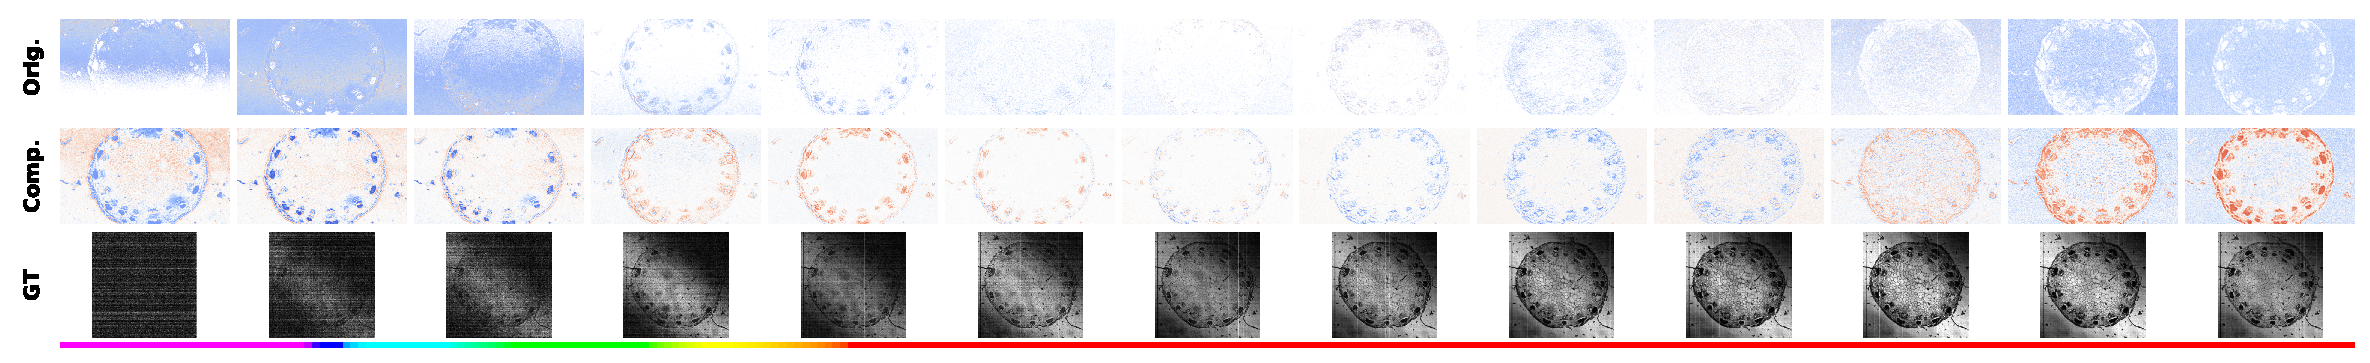
\includegraphics[width=0.98\textwidth]{../../publication_code/figures/figure04_allinone_20251101_161009/figure04_rescaled_grid_bins_03_15.pdf}
% 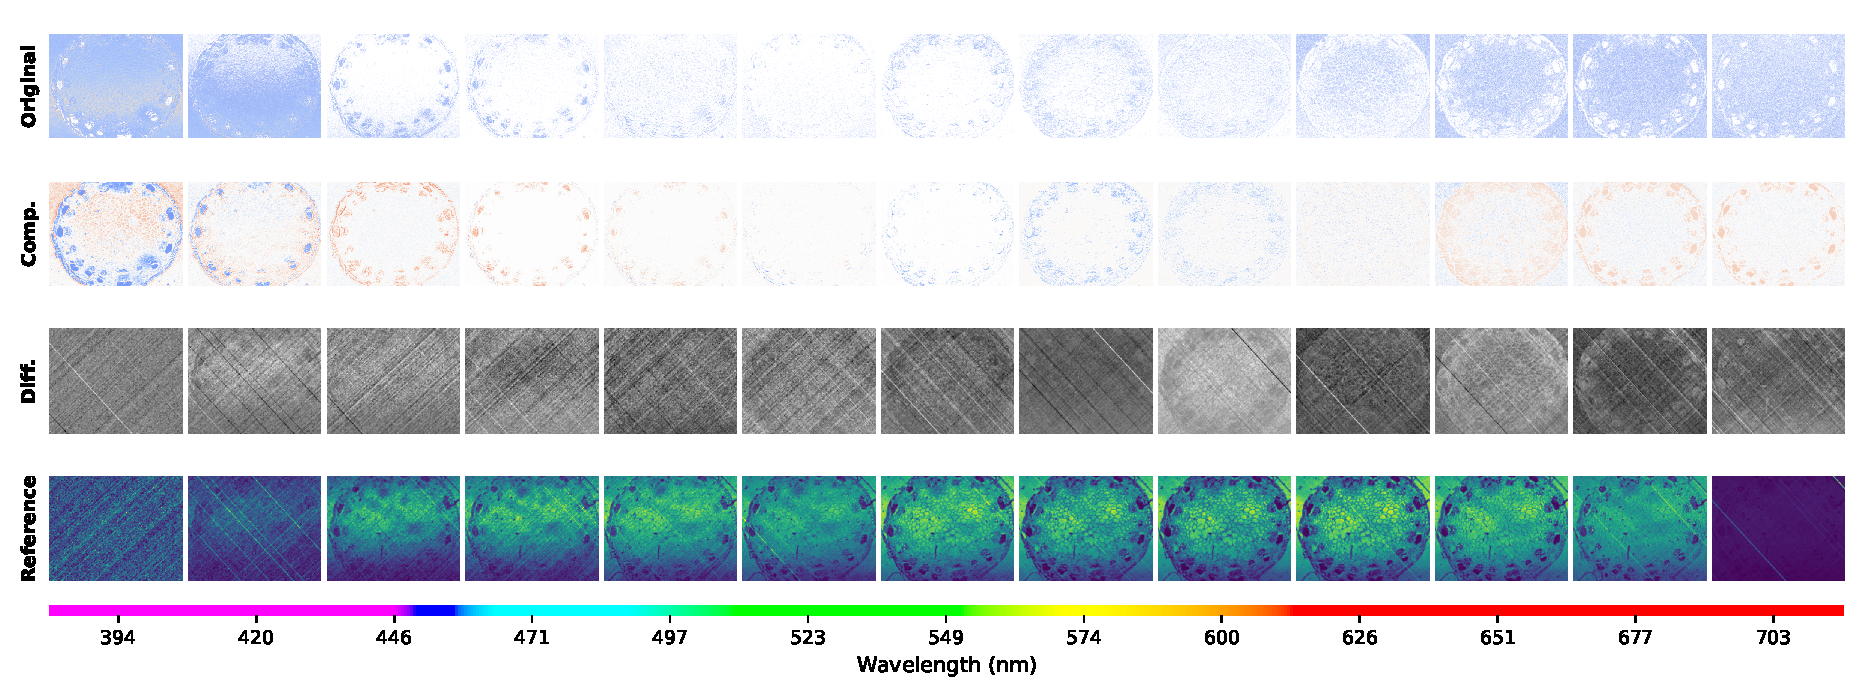
\includegraphics[width=0.98\textwidth]{figures/spectral_reconstruction_scan_rotated_cropped_400_700.pdf}
%   \caption{
%   % Spectral reconstruction across a single forward scan. Each column shows a 50~ms temporal bin.
%    % (top: original; bottom: compensated with 3$\times$3$\times$3 smoothing and background subtraction). 
%    Spectral reconstruction across a single forward scan. The view spans 175--775~ms (\(\approx 390\) to 660~nm). Columns sample five 50~ms bins centred near 389, 456, 523, 590, and 657~nm. Rows (top to bottom): original cumulative events, multi-window compensated accumulation, 20~nm wavelength-gradient slices from the reference hyperspectral camera, and the 300~s reference exposure.
%    }
%   \label{fig:spectrum}
% \end{figure*}

\olsection{System architecture and sensing model}
Figure~\ref{fig:overview} sketches the optical layout. A broadband LED source passes through a slit and diffraction grating before illuminating the specimen. The transmitted light is collected by a microscope and relayed through a 4$f$ system onto a hybrid detection plane comprising an event camera and a frame camera. The motor executes repeated forward/backward scans, but its speed is neither constant nor calibrated.

Under small-angle assumptions the wavelength incident on pixel $(x,y)$ is
\begin{equation}
  \lambda(x,t) \approx d\!\left(\frac{x}{z_2} - \frac{\xi(t)}{z_1}\right),
  \label{eq:lambda_mapping}
\end{equation}
where $d$ is the grating dispersion constant, $z_2$ and $z_1$ denote distances from the grating to the sensor and illumination relay, and $\xi(t)$ is the motor displacement inferred from the data stream. The transmitted intensity can be written as $I_{x,y}(t) = I_0^{(x,y)}[\lambda(x,t)]$, leading to the temporal gradient
\begin{equation}
  \frac{\partial I_{x,y}}{\partial t} = \frac{\partial I_0^{(x,y)}}{\partial \lambda} \frac{\partial \lambda(x,t)}{\partial t},
  \label{eq:intensity_gradient}
\end{equation}
which drives event emission when the logarithmic intensity crosses the sensor threshold. Because $\partial \lambda/\partial t$ is governed by the motor trajectory, reconstructing $I_0^{(x,y)}(\lambda)$ reduces to integrating polarity-weighted events along a synchronized wavelength axis.

\begin{figure}[t]
  \centering
  \begin{tikzpicture}
    \node[anchor=south west, inner sep=0] (f2b) at (0,0)
      % {\includegraphics[width=\linewidth]{../../publication_code/figures/figure02_correlation.pdf}};
      {\includegraphics[width=0.8\linewidth]{figures/figure02_correlation.pdf}};
    \begin{scope}[x={(f2b.south east)}, y={(f2b.north west)}]
      \node[font=\bfseries, anchor=north west, fill=none, text=black, inner sep=2pt] at (0.0, 1.05) {(a)};
    \end{scope}
  \end{tikzpicture}\\[-10pt]
  % \vspace{-10pt}
  \begin{tikzpicture}
    \node[anchor=south west, inner sep=0] (f2a) at (0,0)
      % {\includegraphics[width=\linewidth]{../../publication_code/figures/figure02_activity.pdf}};
      {\includegraphics[width=0.8\linewidth]{figures/figure02_activity.pdf}};
    \begin{scope}[x={(f2a.south east)}, y={(f2a.north west)}]
      \node[font=\bfseries, anchor=north west, fill=none, text=black, inner sep=2pt] at (0.0, 1.05) {(b)};
    \end{scope}
  \end{tikzpicture}\\[-10pt]
  % \vspace{-10pt}
  \caption{Self-synchronized scan segmentation. (a) Auto-correlation and auto-convolution of the event activity signal; the red and blue marker indicates the peak used to determine the period, start and end of scanning. (b) Event counts over the full recording with pre- and post-scan shading and alternating forward and backward boundaries. }
  \label{fig:segmentation}
\end{figure}

\begin{figure}[t]
  \centering
  % (a) 3D event cloud before compensation
  \begin{tikzpicture}
    \node[anchor=south west, inner sep=0] (img3a) at (0,0)
      {\includegraphics[width=1\linewidth]{figures/event_cloud_before.pdf}};
    \begin{scope}[x={(img3a.south east)}, y={(img3a.north west)}]
      \node[font=\bfseries, anchor=north west, fill=none, text=black, inner sep=2pt]
        at (-0.05, 1.050) {(a)};
      % Discrete polarity legend using dot handles (−1 light blue, +1 orange)
      \def\lx{0.70}\def\ly{0.92}\def\rr{0.014}
      \filldraw[fill=evtNeg, draw=black, line width=0.2pt] (\lx,\ly) circle (\rr);
      \node[anchor=west, inner sep=1pt, scale=0.7] at (\lx+0.03, \ly) {$-1$};
      \filldraw[fill=evtPos, draw=black, line width=0.2pt] (\lx,\ly-0.06) circle (\rr);
      \node[anchor=west, inner sep=1pt, scale=0.7] at (\lx+0.03, \ly-0.06) {$+1$};
    \end{scope}
  \end{tikzpicture}\\[-8pt]

  % (b) 3D event cloud after compensation
  \begin{tikzpicture}
    \node[anchor=south west, inner sep=0] (img3b) at (0,0)
      {\includegraphics[width=1\linewidth]{figures/event_cloud_after.pdf}};
    \begin{scope}[x={(img3b.south east)}, y={(img3b.north west)}]
      \node[font=\bfseries, anchor=north west, fill=none, text=black, inner sep=2pt]
        at (-0.05, 1.050) {(b)};
    \end{scope}
  \end{tikzpicture}\\[-4pt]

  % (c,d) 50 ms accumulations, side-by-side, with external color bar to the right of (d)
  \begin{minipage}[t]{0.465\linewidth}
    \begin{tikzpicture}
      \node[anchor=south west, inner sep=0] (img3c) at (0,0)
        {\includegraphics[width=\linewidth]{figures/overlay_image_before_plain.pdf}};
      \begin{scope}[x={(img3c.south east)}, y={(img3c.north west)}]
        \node[font=\bfseries, anchor=north west, fill=none, text=black, inner sep=2pt]
          at (-0.05, 1.12) {(c)};
      \end{scope}
    \end{tikzpicture}
  \end{minipage}\hspace{0.012\linewidth}
  \begin{minipage}[t]{0.465\linewidth}
    \begin{tikzpicture}
      \node[anchor=south west, inner sep=0] (img3d) at (0,0)
        {\includegraphics[width=\linewidth]{figures/overlay_image_after_plain.pdf}};
      \begin{scope}[x={(img3d.south east)}, y={(img3d.north west)}]
        \node[font=\bfseries, anchor=north west, fill=none, text=black, inner sep=2pt]
          at (-0.05, 1.12) {(d)};
      \end{scope}
    \end{tikzpicture}
  \end{minipage}\hspace{0.012\linewidth}
  % External color bar to the right of (d): light blue -> white -> orange
  \begin{minipage}[t]{0.06\linewidth}
    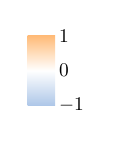
\begin{tikzpicture}
      \begin{scope}
        \def\xb{0.10}\def\yb{0.06}\def\wb{0.35}\def\hb{0.88}
        \shade[bottom color=evtNeg, top color=white] (\xb,\yb) rectangle (\xb+\wb, \yb+0.5*\hb);
        \shade[bottom color=white, top color=evtPos] (\xb,\yb+0.5*\hb) rectangle (\xb+\wb, \yb+\hb);
        \node[anchor=west, inner sep=1pt, scale=0.7] at (\xb+\wb+0.02, \yb) {$-1$};
        \node[anchor=west, inner sep=1pt, scale=0.7] at (\xb+\wb+0.02, \yb+0.5*\hb) {$0$};
        \node[anchor=west, inner sep=1pt, scale=0.7] at (\xb+\wb+0.02, \yb+\hb) {$1$};
      \end{scope}
    \end{tikzpicture}
  \end{minipage}\\[-2pt]

  \caption{Multi-window scanning compensation results. Panels (a) and (b) show 3D event clouds before and after compensation, respectively. In each, a semi-transparent panel with a dashed outline (red in (a), green in (b)) marks the spatial footprint of a short (50~ms) temporal accumulation range. Panels (c) and (d) present the corresponding 2D event accumulations over that same range (before and after), matching the marked regions in (a) and (b). A polarity legend (\mbox{$-1$}, \mbox{$+1$}) is shown in (a); a continuous intensity color bar for (c,d) appears beside (d).}
  \label{fig:warp}
\end{figure}

% \begin{figure*}[t]
%   \centering
%   % 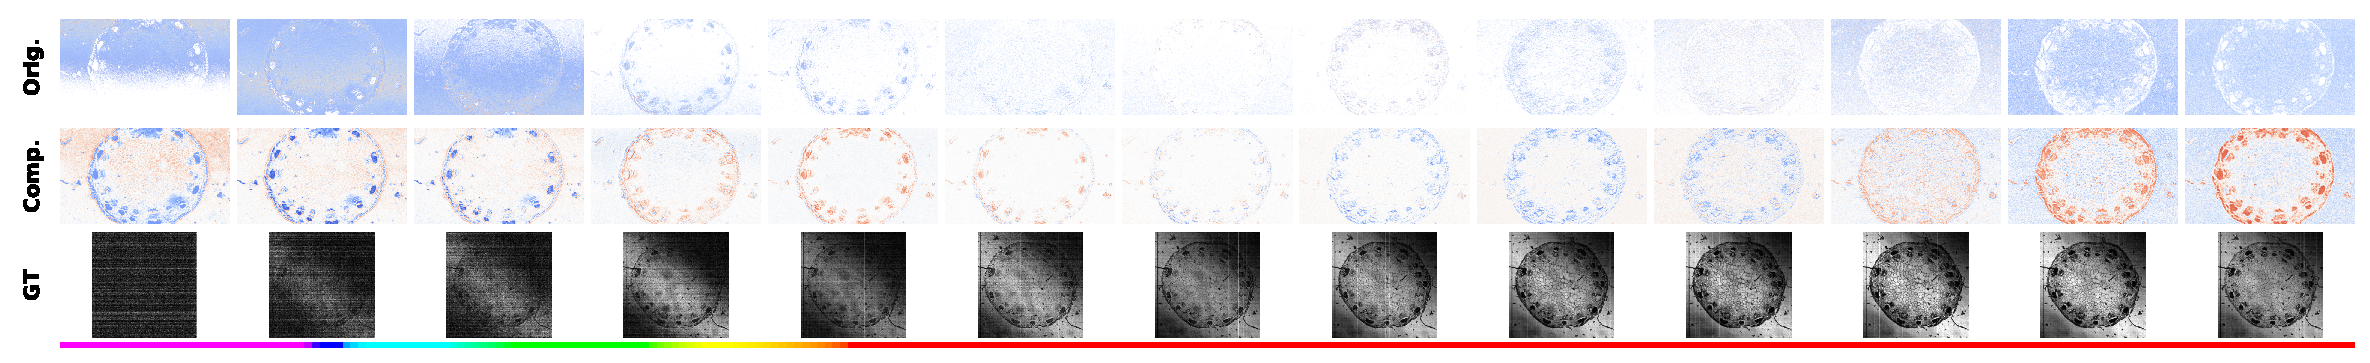
\includegraphics[width=0.98\textwidth]{../../publication_code/figures/figure04_allinone_20251101_161009/figure04_rescaled_grid_bins_03_15.pdf}
% 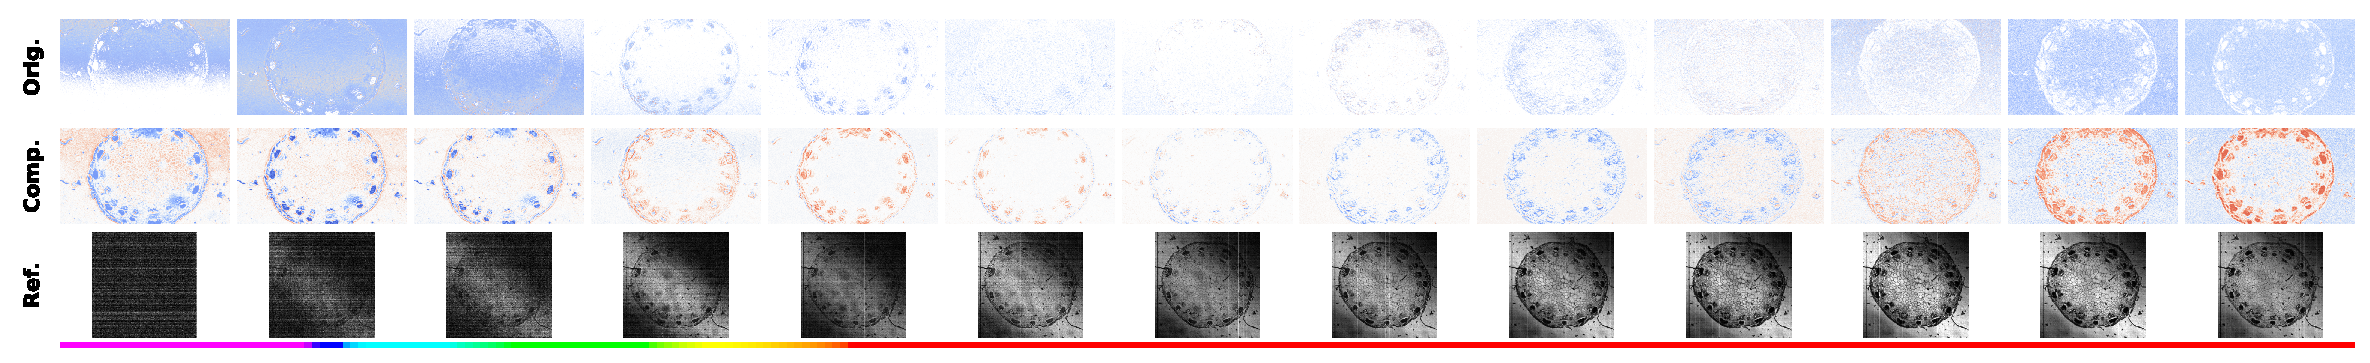
\includegraphics[width=0.98\textwidth]{figures/figure04_rescaled_grid_bins_03_15.pdf}
%   \caption{
%   Spectral reconstruction across a single forward scan. Each column shows a 50~ms temporal bin.
%    % (top: original; bottom: compensated with 3$\times$3$\times$3 smoothing and background subtraction). 
%    }
%   \label{fig:spectrum}
% \end{figure*}

\begin{figure*}[t]
  \centering
  % 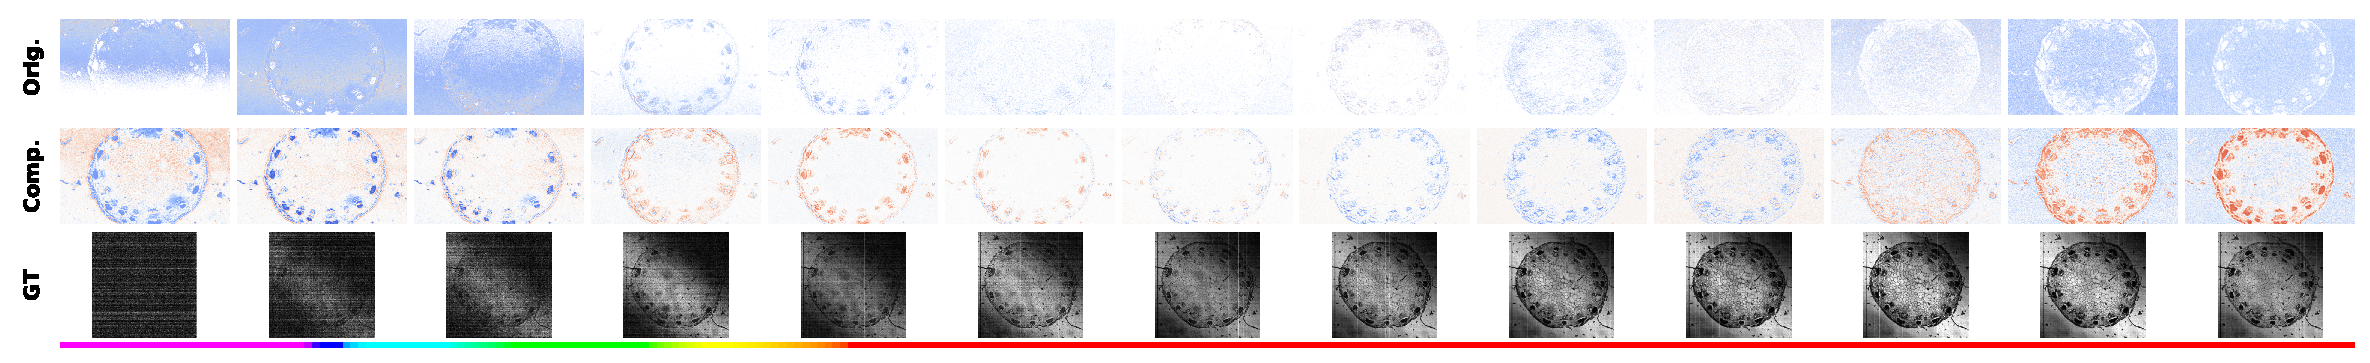
\includegraphics[width=0.98\textwidth]{../../publication_code/figures/figure04_allinone_20251101_161009/figure04_rescaled_grid_bins_03_15.pdf}
\includegraphics[width=0.98\textwidth]{figures/spectral_reconstruction_coolwarm.pdf}\\[-0pt]
  \caption{
  % Spectral reconstruction across a single forward scan. Each column shows a 50~ms temporal bin.
   % (top: original; bottom: compensated with 3$\times$3$\times$3 smoothing and background subtraction). 
   Spectral reconstruction across a single forward scan. The view spans 175--775~ms (\(\approx 390\) to 660~nm). Columns sample five 50~ms bins centred near 389, 456, 523, 590, and 657~nm. Rows (top to bottom): original cumulative events, multi-window compensated accumulation, 20~nm wavelength-gradient slices from the reference hyperspectral camera, and the 300~s reference exposure.
   }
  \label{fig:spectrum}
\end{figure*}

\olsection{Self-synchronized scan segmentation}
Event timestamps are binned (1~ms) into an activity trace. Two correlation peaks anchor the segmentation: the dominant auto-correlation peak gives the round-trip period, and the strongest reverse-correlation peak fixes the symmetric turnaround, which jointly set the pre-scan, main scan, and post-scan spans. A brief iterative refinement repeats the peak search after updating these spans, stabilising the forward/backward boundaries without external triggers (full formulas in the Supplementary Material). This data-driven procedure adapts to slow drifts and produces consistent temporal support for all reconstructions. 
% Planned figs include (i) using only the first forward/back pair to quantify baseline noise, and (ii) averaging all three pairs to demonstrate variance reduction. 

\olsection{Multi-window scanning compensation}
Even with accurate segmentation, \eqref{eq:lambda_mapping} introduces a spatially varying delay through the $x/z_2$ term; motor acceleration near turnarounds further shears the time axis. Our multi-window compensation routine addresses this by fitting boundary surfaces
\begin{equation}
  T_i(x,y) = a_i x + b_i y + c_i,
\end{equation}
which partition each scan into $M$ temporal windows. Soft memberships,
\begin{equation}
  w_i(x,y,t) = \frac{\sigma\!\left(\frac{t - T_i}{\tau}\right)\sigma\!\left(\frac{T_{i+1}-t}{\tau}\right)}{\sum_j \sigma\!\left(\frac{t - T_j}{\tau}\right)\sigma\!\left(\frac{T_{j+1}-t}{\tau}\right)},
\end{equation}
blend adjacent windows (temperature $\tau \approx 1$~ms). The compensated time is
\begin{equation}
  t' = t - \sum_{i=1}^{M-1} w_i(x,y,t)\bigl(\tilde{a}_i x + \tilde{b}_i y \bigr),
  \label{eq:timewarp}
\end{equation}
where $\{\tilde{a}_i,\tilde{b}_i\}$ are trainable slopes optimized by minimizing the spatial variance of binned event intensities while enforcing smoothness across neighbouring windows. The objective is 
\begin{equation}
\begin{split}
  \mathcal{L}(\theta)
  &= 
  \underbrace{
  \tfrac{1}{HW}\!\sum_k\!\sum_{x,y}
  \bigl(\mathsf{E}_k(x,y;\theta)-\mu_k\bigr)^2
  }_{\mathcal{L}_{\mathrm{var}}} \\[3pt]
  &\quad + 
  \lambda_{\mathrm{sm}}
  \underbrace{
  \sum_{i=1}^{M-2}
  \!\Big[
  (\tilde{a}_{i+1}-\tilde{a}_i)^2
  +(\tilde{b}_{i+1}-\tilde{b}_i)^2
  \Big]
  }_{\mathcal{L}_{\mathrm{sm}}},
  \label{eq:loss}
\end{split}
\end{equation}
where $\mu_k = (HW)^{-1}\sum_{x,y}\mathsf{E}_k(x,y;\theta)$ and $\lambda_{\mathrm{sm}}$ controls the smoothness strength. Minimizing $\mathcal{L}(\theta)$ by gradient descent aligns temporal windows, suppresses acceleration-induced shear, and yields sharper spectral reconstructions than a single-plane warp.

Figure~\ref{fig:warp} summarizes the effects of the proposed multi-window compensation of one scanning segment. 
Panel~(a) illustrates how the learned boundary surfaces align the event distribution in both spatial--temporal projections, effectively capturing the nonuniform scanning motion. 
The fitted slopes span from  \SI{-1.74}{\micro\second\per\pixel} to \SI{5.50}{\micro\second\per\pixel} for \(a\), and from \SI{-79.82}{\micro\second\per\pixel} to \SI{-75.67}{\micro\second\per\pixel} for \(b\), , representing the lateral and vertical time-per-pixel coefficients of the multi-window model.
Panel~(b) shows that the temporal variance within each 50~ms bin decreases after compensation, indicating improved temporal coherence across the field of view. 
Panel~(c) compares representative cumulative event frames before and after correction, where the removal of diagonal blur patterns confirms that the time-warp model successfully restores the spatial integrity of each spectral slice.

\begin{figure}[t]
  \centering
  % Single aligned overlay (Background vs Groundtruth)
  % \includegraphics[width=\columnwidth]{../../publication_code/figures/figure04_allinone_20251103_214813/figure04_rescaled_bg_gt_third_only.png}
  \includegraphics[width=\columnwidth]{figures/figure04_edges_only_third.pdf}\\[-10pt]
  \caption{Aligned background mapped to wavelength using the auto-alignment (\SIrange{400}{700}{\nano\meter} $\approx$ \SIrange{236}{821}{\milli\second} in
  the background timeline) compared against a single spectrometer curve. }
  \label{fig:figure5}
\end{figure}

\olsection{Time--wavelength auto-alignment}
A one-dimensional background trace $b(t)$ is computed from polarity-weighted, fast-compensated events using a fixed step $\Delta t$ (5~ms). After normalising by the start and end plateaus,
\begin{equation}
  \tilde b(t)=\frac{b(t)-\mu_{\mathrm{pre}}}{\mu_{\mathrm{post}}-\mu_{\mathrm{pre}}},\quad t\in[0,T],
\end{equation}
the active scan interval $[t_0,t_1]$ is identified from rising and falling edge quantiles of the smoothed $\tilde b(t)$ (definitions in Supplementary Material). For ground-truth spectra $\{g_i(\lambda)\}_{i=1}^M$ with active intervals $[\lambda_{0,i},\lambda_{1,i}]$, the time-to-wavelength mapping is given by the affine model
\begin{equation}
  \lambda(t)=\alpha t+\beta,\quad 
  \alpha=\frac{\bar\lambda_1-\bar\lambda_0}{t_1-t_0},\;
  \beta=\bar\lambda_0-\alpha t_0,
\end{equation}
where $\bar\lambda_0$ and $\bar\lambda_1$ are the mean boundary wavelengths across curves. The transformed series $\tilde b_\lambda(\lambda)=\tilde b\big((\lambda-\beta)/\alpha\big)$ is then amplitude-aligned to the mean ground-truth $\bar g(\lambda)=M^{-1}\sum_i \tilde g_i(\lambda)$ by a least-squares affine fit,
\begin{equation}
  (a^*,c^*)=\arg\min_{a,c}\sum_j[\bar g(\lambda_j)-a\,\tilde b_\lambda(\lambda_j)-c]^2,
\end{equation}
with closed-form solution $[a^*,c^*]^\top=(X^\top X)^{-1}X^\top\mathbf{y}$, $X=[\tilde b_\lambda\;\mathbf{1}]$, $\mathbf{y}=\bar g$. Symbol definitions (edge levels, $t_0,t_1$) are listed in the Supplementary Material.

Figure~\ref{fig:figure5} shows the background alignment result, where the event-derived wavelength mapping agrees closely with the spectrometer reference curve.


\olsection{Spectral reconstruction and benchmarking}
After compensation, events are cumulated along $t'$ into quasi-static frames $\mathsf{E}_k(x,y)$, with each cumulative window advanced by a \SI{5}{\milli\second} temporal step, and polarity-weighted counts integrated to recover relative spectra. Figure~\ref{fig:spectrum} illustrates the reconstructed spectral sequence across a single forward scan, showing the temporal evolution of wavelength-dependent features derived from the event stream.
Table~\ref{tab:acquisition_comparison} summarizes the acquisition time and cost differences between the proposed event-driven system and a conventional frame-based hyperspectral camera. 
Under the same illumination condition, our event-driven system completes a full spectral scan within \SIrange{150}{1100}{\milli\second}, whereas the reference hyperspectral camera requires approximately \SI{300}{\second} for an equivalent acquisition. 
All structural components of our prototype are 3D printed using an Ultimaker~3S printer, while the optical and mechanical parts include a diffraction grating priced at about \SI{1.3}{\USD} and a motor--controller set costing approximately \SI{32.5}{\USD}. The total material cost of the complete event hyperspectral system is therefore below \SI{35}{\USD}. 
In addition to the drastic reduction in acquisition time and cost, the asynchronous sensing architecture offers high dynamic range and resilience to illumination fluctuations, maintaining reliable performance even in low-light environments where the frame-based camera exhibits noise saturation and motion blur. 
These results highlight the efficiency and practicality of self-synchronized, event-based hyperspectral imaging for compact and adaptive optical platforms.

\begin{table}[t]
\centering
\caption{Acquisition time and cost comparison between the proposed event-driven system and a reference hyperspectral camera.}
\label{tab:acquisition_comparison}
\begin{tabular}{lcc}
\hline
\textbf{Parameter} & \textbf{Ours} & \textbf{Reference camera} \\
\hline
Acquisition time & $\sim$\SI{1100}{\milli\second} per scan & \SI{300}{\second} per scan \\
Approx.\ price & $\sim$\SI{3000}{\USD} & \SI{14000}{\USD} \\
\hline
\end{tabular}
\end{table}

\olsection{Discussion and outlook}
The self-synchronizing strategy removes the need for encoder calibration while tolerating speed fluctuations from cost-effective actuators, distinguishing this platform from prior systems that assumed precise timing hardware~\cite{hagen2013review,yeh2011selfcal}. The variance-minimizing, multi-window time warp extends piecewise-affine compensations used in event-based motion estimation~\cite{mitrokhin2018mobility}, adapting them to the spectral scanning context. Together these components enable transmission-mode spectral capture without illumination modulation or auxiliary sensors.

% Planned figures: (i) gather datasets spanning single and triple scan fusion to populate Fig.~\ref{fig:segmentation}(d); (ii) quantify variance reduction and residual blur for multi-window versus single-plane warps to complete Fig.~\ref{fig:warp}; and (iii) collect spectral overlays under nominal and low-light scenarios to fill Fig.~\ref{fig:spectrum}. 

\olsection{Conclusion}
We presented a self-synchronized, event-driven transmission hyperspectral system that derives scan timing from the event stream and compensates temporal shear using a multi-window time warp. Despite relying on inexpensive, non-uniform motor motion, the reconstructed spectra align with a reference hyperspectral camera and retain fidelity under reduced illumination. 

\begin{backmatter}
\bmsection{Funding}
The work was supported by the Research Grants Council of Hong Kong (GRF 17201822 and RIF R7003-21).

\bmsection{Acknowledgment}

\bmsection{Disclosures}
The authors declare no conflicts of interest.

\bmsection{Data Availability}
Data underlying the results presented in this paper are available from the corresponding author upon reasonable request. All 3D-printable components, design files, and source code used in this work are openly accessible at the provided GitHub repository.
\end{backmatter}


\bibliography{ref}

\end{document}
